\section{最优性的判别}
\label{sec:ot-optimality}

图~\ref{fig:ot-plan-tables}(c)的逐格搬运成本是$0.6$。怎样确信没有更便宜的方案？逐个比较做不到，可行方案有无穷多个。每个可行方案只给出最优值的一个上界；要证实某个方案最优，还需要一个对一切可行方案都成立的下界，并且它恰好等于这个方案的成本。本节先构造这样的下界，再说明它在什么条件下能与原问题的最优值相等。

\subsection{对偶势}
\label{sec:ot-potentials}

先在有限情形找下界。设想有人提出一组价格：在源位置$x_i$交出一份质量可得收入$f_i$，在目标位置$y_j$收下一份质量可得收入$g_j$。若价格满足
\[
 f_i+g_j\leq c_{i,j}\qquad\text{对一切}\ i,j ,
\]
则无论按什么方案搬运，每份质量带来的收入都不超过它的运费。把行和约束乘以$f_i$、列和约束乘以$g_j$再相加，对任意$\bm{\pi}\in U(\bm{a},\bm{b})$，
\[
 \sum_ia_if_i+\sum_jb_jg_j=\sum_{i,j}\pi_{i,j}(f_i+g_j)\leq\sum_{i,j}\pi_{i,j}c_{i,j} .
\]
左边不依赖方案，所以它是所有可行方案成本的一个公共下界。一般分布的写法相同，只是把向量换成函数。

\begin{definition}[对偶势]
\label{def:ot-potentials}
设$\mu,\nu$与成本$c\geq0$如定义~\ref{def:ot-problem}。若$\varphi\in L^{1}(\mu)$，$\psi\in L^{1}(\nu)$，并且
\begin{equation}
 \varphi(x)+\psi(y)\leq c(x,y)\qquad\text{对一切}\ x\in\mathcal{X},\ y\in\mathcal{Y},
 \label{eq:ot-dual-constraint}
\end{equation}
则称$(\varphi,\psi)$为一对可行的\term{对偶势}（dual potentials），称
\begin{equation}
 J(\varphi,\psi)=\int\varphi\,\mathrm{d}\mu+\int\psi\,\mathrm{d}\nu
 \label{eq:ot-dual-value}
\end{equation}
为它的对偶值。
\end{definition}

对偶势里的$\varphi,\psi$可以取负值，只要求可积；这样它们的积分有限，后面的相减才有意义。下面的定理把“价格”论证写成一般形式，并且给出原对偶值之差的精确表达式。

\begin{theorem}[弱对偶与原对偶差]
\label{thm:ot-weak-duality}
设$(\varphi,\psi)$是可行的对偶势，$\pi\in\Pi(\mu,\nu)$。则
\begin{equation}
 \int c\,\mathrm{d}\pi-J(\varphi,\psi)=\int\bigl(c(x,y)-\varphi(x)-\psi(y)\bigr)\,\pi(\mathrm{d}x,\mathrm{d}y)\geq0 ,
 \label{eq:ot-gap}
\end{equation}
两边可以同时为$+\infty$。于是$J(\varphi,\psi)\leq\operatorname{OT}_c(\mu,\nu)$。若某个$\pi$与$(\varphi,\psi)$使式~\eqref{eq:ot-gap}为零，则$\pi$是最优耦合，$(\varphi,\psi)$使对偶值最大。
\end{theorem}

\begin{proof}
由于$\pi$的第一边缘是$\mu$，对可积的$\varphi$有
\[
 \int\varphi(x)\,\pi(\mathrm{d}x,\mathrm{d}y)=\int\varphi\,\mathrm{d}\mu .
\]
这对示性函数是边缘的定义，对简单函数由线性性成立，对非负函数由单调收敛定理成立，再对正负部分分别使用即得可积情形。$\psi$同理。

记松弛量$s(x,y)=c(x,y)-\varphi(x)-\psi(y)$，由式~\eqref{eq:ot-dual-constraint}它非负，积分有定义。$c=s+\varphi+\psi$中后两项关于$\pi$可积，所以
\[
 \int c\,\mathrm{d}\pi=\int s\,\mathrm{d}\pi+\int\varphi\,\mathrm{d}\mu+\int\psi\,\mathrm{d}\nu ,
\]
这就是式~\eqref{eq:ot-gap}。对$\pi$取下确界得$J(\varphi,\psi)\leq\operatorname{OT}_c(\mu,\nu)$。若差为零，$\pi$的成本等于一个下界，不可能有成本更低的耦合；对任何别的可行对偶势$(\varphi',\psi')$，由刚证明的不等式，$J(\varphi',\psi')$不超过$\int c\,\mathrm{d}\pi$，而后者等于$J(\varphi,\psi)$。
\end{proof}

式~\eqref{eq:ot-gap}的右边只看$\pi$把质量放在哪里：放在松弛量为零的地方不贡献差，放在松弛量为正的地方按松弛量计差。所以候选方案$\pi$的最优性可以这样核验：找一对可行的对偶势，检查$\pi$的质量是否几乎全部落在等号集合$\{c=\varphi+\psi\}$上。这一条件称为互补松弛。

\paragraph{例子的证据}
回到全章例子。取
\[
 \bm{f}=(0,\ -1,\ -2),\qquad \bm{g}=(0,\ 1,\ 2),
\]
则$f_i+g_j=j-i$。成本$(i-j)^{2}$与它的差就是松弛矩阵
\[
 \bm{S}=\bm{C}-\bigl(f_i+g_j\bigr)_{i,j}=\begin{bmatrix}0&0&2\\2&0&0\\6&2&0\end{bmatrix}.
\]
各元素非负，所以$(\bm{f},\bm{g})$可行；对偶值为
\[
 \langle\bm{a},\bm{f}\rangle+\langle\bm{b},\bm{g}\rangle=(-0.3-0.4)+(0.3+1.0)=0.6 .
\]
逐格搬运的质量放在$(0,0),(0,1),(1,2),(2,2)$上，这四处的松弛量都是$0$，于是它的成本$0.6$等于这个下界，它是最优方案。

同一对势也给出其他方案离最优有多远。由式~\eqref{eq:ot-gap}，跳格搬运把$0.3$放在松弛量为$2$的$(0,2)$处，所以
\[
 1.2-0.6=0.3\times2 .
\]
独立方案在每个格子上都有质量，它与最优值之差是$\sum_{i,j}a_ib_js_{i,j}$，逐项相加得
\[
 0.25\times2+0.06\times2+0.04\times6+0.06\times2=0.98=1.58-0.6 .
\]
图~\ref{fig:ot-dual-envelope}(b)画出松弛矩阵，红圈标出最优方案的质量所在。

\paragraph{由一个势求另一个势}
给定$\bm{g}$，满足约束的$f_i$最大能取多少？约束$f_i\leq c_{i,j}-g_j$对每个$j$成立，所以最大可取
\begin{equation}
 f_i=\min_{j}\bigl(c_{i,j}-g_j\bigr).
 \label{eq:ot-c-transform}
\end{equation}
这称为$\bm{g}$的\term{$c$变换}（$c$-transform）；一般情形写成$\psi^{c}(x)=\inf_y\bigl(c(x,y)-\psi(y)\bigr)$。对偶值关于$\bm{f}$单调增加，所以最优的$\bm{f}$总可以取成$\bm{g}$的$c$变换。几何上，它是一族曲线$x\mapsto c(x,y_j)-g_j$的下包络。图~\ref{fig:ot-dual-envelope}(a)对例子中的$\bm{g}=(0,1,2)$画出三条抛物线$(x-j)^{2}-j$与它们的下包络，在$x=0,1,2$处恰好取到$\bm{f}=(0,-1,-2)$。

\begin{BookInlineFigure}
 \centering
 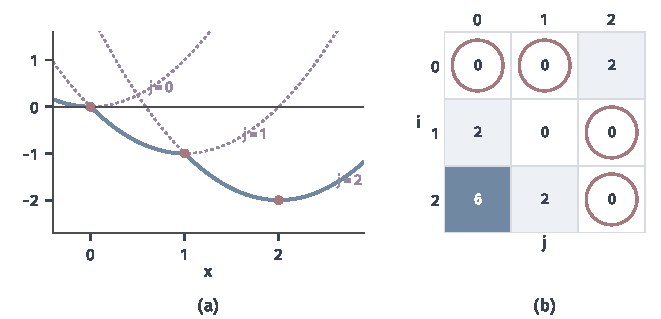
\includegraphics[width=112mm]{figures/07-probability/07-distribution-optimization/matplotlib/ot-dual-envelope/figure.pdf}
 \caption{全章例子的对偶势。(a)紫色点线是$(x-j)^{2}-g_j$，$\bm{g}=(0,1,2)$；蓝线是它们的下包络，即$\bm{g}$的$c$变换；红点是$f_i$。(b)松弛量$c_{i,j}-f_i-g_j$，红圈是逐格搬运方案的非零位置，全部落在零松弛处。}
 \label{fig:ot-dual-envelope}
\end{BookInlineFigure}

成本取度量$d$时，$c$变换产生第~\ref{chap:distribution-comparison}章的Lipschitz函数：$\psi^{c}(x)=\inf_y(d(x,y)-\psi(y))$是一族$1$-Lipschitz函数的下确界，本身也是$1$-Lipschitz函数。再对一个$1$-Lipschitz函数$h$求$c$变换，由$h(y)-h(x)\leq d(x,y)$得$\inf_y(d(x,y)-h(y))\geq-h(x)$，取$y=x$取等，结果恰为$-h$。所以对偶势可以取成$(-h,h)$的形式，对偶值是$\mathbb{E}_{\nu}[h]-\mathbb{E}_{\mu}[h]$；Kantorovich--Rubinstein对偶正是一般对偶在$c=d$时的这一特殊形式。

最优势一般不唯一。例子中把$\bm{f}$加上常数$t$、$\bm{g}$减去$t$，对偶值不变；即使固定$f_0=0$，可行最优势也不止一组。由零松弛的四个位置得$g_0=0$，$g_1=1$，$g_2=1-f_1$，$f_2=f_1-1$，再检查其余五个约束，得到$-3\leq f_1\leq-1$，其中每个$f_1$都给出对偶值$0.6$。最优方案唯一（第~\ref{sec:ot-one-dimensional}节将证明），证明它最优的价格却有许多组。

\subsection{强对偶的条件}
\label{sec:ot-strong-duality}

弱对偶只给出不等式。要用对偶势证实最优性，还需要知道下界能够逼近甚至等于最优值，即两个问题之间没有\term{对偶间隙}（duality gap）。先证明有限情形。

\begin{theorem}[有限运输问题的强对偶]
\label{thm:ot-finite-duality}
设$\bm{a}\in\mathbb{R}^{m}$，$\bm{b}\in\mathbb{R}^{n}$是概率向量，$\bm{C}\in\mathbb{R}^{m\times n}$。则
\begin{equation}
 \min_{\bm{\pi}\in U(\bm{a},\bm{b})}\langle\bm{C},\bm{\pi}\rangle=\max\Bigl\{\langle\bm{a},\bm{f}\rangle+\langle\bm{b},\bm{g}\rangle:\ f_i+g_j\leq c_{i,j}\ \text{对一切}\ i,j\Bigr\},
 \label{eq:ot-finite-duality}
\end{equation}
两边的最小值与最大值都能取到。
\end{theorem}

\begin{proof}
把$\bm{\pi}$的$mn$个元素看成变量。原问题是线性规划：在等式约束$\sum_j\pi_{i,j}=a_i$（$m$个）、$\sum_i\pi_{i,j}=b_j$（$n$个）和$\pi_{i,j}\geq0$下最小化$\sum_{i,j}c_{i,j}\pi_{i,j}$。给前$m$个等式配乘子$f_i$，后$n$个配乘子$g_j$，Lagrange函数是
\[
 \sum_{i,j}c_{i,j}\pi_{i,j}+\sum_if_i\Bigl(a_i-\sum_j\pi_{i,j}\Bigr)+\sum_jg_j\Bigl(b_j-\sum_i\pi_{i,j}\Bigr).
\]
整理成
\[
 \langle\bm{a},\bm{f}\rangle+\langle\bm{b},\bm{g}\rangle+\sum_{i,j}\bigl(c_{i,j}-f_i-g_j\bigr)\pi_{i,j} .
\]
对$\pi_{i,j}\geq0$取下确界，只有当每个系数$c_{i,j}-f_i-g_j$都非负时下确界才有限，等于$\langle\bm{a},\bm{f}\rangle+\langle\bm{b},\bm{g}\rangle$。所以对偶线性规划正是式~\eqref{eq:ot-finite-duality}右边。

原问题可行（含$\bm{a}\bm{b}^{\top}$），目标值不小于$\min_{i,j}c_{i,j}$，有下界。由线性规划的强对偶定理，原问题与对偶问题都有最优解，并且最优值相等，可参考\BookChapterRef{chap:linear-programming}{卷五第2章“线性规划”}。
\end{proof}

第~\ref{chap:distribution-comparison}章证明有限支撑的Kantorovich--Rubinstein对偶，用的正是这个定理。一般分布不能直接套用线性规划，但在紧致空间上可以用有限问题去逼近。

\begin{theorem}[紧致空间上的强对偶]
\label{thm:ot-compact-duality}
设$(\mathcal{X},d_{\mathcal{X}})$，$(\mathcal{Y},d_{\mathcal{Y}})$是紧致度量空间，$c:\mathcal{X}\times\mathcal{Y}\to[0,\infty)$连续，$\mu,\nu$分别是其上的Borel概率分布。则
\begin{equation}
 \operatorname{OT}_c(\mu,\nu)=\sup\bigl\{J(\varphi,\psi):\ (\varphi,\psi)\ \text{是有界可测的可行对偶势}\bigr\}.
 \label{eq:ot-compact-duality}
\end{equation}
\end{theorem}

\begin{proof}
由定理~\ref{thm:ot-weak-duality}，右边不超过左边，只需对每个$\eta>0$构造对偶值不小于$\operatorname{OT}_c(\mu,\nu)-3\eta$的可行势。

\emph{第一步：选尺度。}$\mathcal{X}\times\mathcal{Y}$紧致，$c$在其上一致连续：存在$\delta>0$，使$d_{\mathcal{X}}(x,x')<\delta$且$d_{\mathcal{Y}}(y,y')<\delta$时$\lvert c(x,y)-c(x',y')\rvert\leq\eta$。

\emph{第二步：离散化。}紧致空间可被有限个半径$\delta/2$的球覆盖，依次去掉与前面重叠的部分并丢弃空集，得到$\mathcal{X}$的有限Borel划分$A_1,\dots,A_m$，每块直径小于$\delta$；同样得到$\mathcal{Y}$的划分$B_1,\dots,B_n$。在每块中取一个代表点$x_i\in A_i$，$y_j\in B_j$，令
\[
 a_i=\mu(A_i),\qquad b_j=\nu(B_j),\qquad c_{i,j}=c(x_i,y_j).
\]
由定理~\ref{thm:ot-finite-duality}，离散问题有最优方案$\bm{\pi}^{\delta}$与最优对偶解$(\bm{f},\bm{g})$，两者的值相等，记为$V_\delta$。

\emph{第三步：离散问题不比原问题贵太多。}把离散方案铺回原空间：在$A_i\times B_j$上放入质量$\pi^{\delta}_{i,j}$，并按$\mu$与$\nu$在这两块上的形状分布，即
\[
 \pi=\sum_{i,j:\ a_i>0,\ b_j>0}\pi^{\delta}_{i,j}\,\frac{\mu|_{A_i}}{a_i}\otimes\frac{\nu|_{B_j}}{b_j} .
\]
（$a_i=0$时第$i$行全为零，可以略去。）由行和$\sum_j\pi^{\delta}_{i,j}=a_i$，它的第一边缘是
\[
 \sum_i\Bigl(\sum_j\pi^{\delta}_{i,j}\Bigr)\frac{\mu|_{A_i}}{a_i}=\sum_i\mu|_{A_i}=\mu ,
\]
第二边缘同理是$\nu$，所以$\pi\in\Pi(\mu,\nu)$。在$A_i\times B_j$上$c\leq c_{i,j}+\eta$，于是
\[
 \operatorname{OT}_c(\mu,\nu)\leq\int c\,\mathrm{d}\pi\leq V_\delta+\eta .
\]

\emph{第四步：把离散势扩展成函数。}令
\[
 \varphi(x)=\min_{j}\bigl(c(x,y_j)-g_j\bigr),\qquad \psi(y)=g_j-\eta\quad(y\in B_j).
\]
$\varphi$是有限个连续函数的最小值，$\psi$是简单函数，都有界可测。可行性：对$y\in B_j$，$\lvert c(x,y_j)-c(x,y)\rvert\leq\eta$，所以
\[
 \varphi(x)+\psi(y)\leq c(x,y_j)-g_j+g_j-\eta\leq c(x,y).
\]
对偶值：对$x\in A_i$，$c(x,y_j)\geq c_{i,j}-\eta$，又由离散对偶可行性$c_{i,j}-g_j\geq f_i$，所以$\varphi(x)\geq f_i-\eta$。于是
\[
 J(\varphi,\psi)\geq\sum_ia_i(f_i-\eta)+\sum_jb_j(g_j-\eta)=V_\delta-2\eta .
\]
与第三步合起来，
\[
 J(\varphi,\psi)\geq\operatorname{OT}_c(\mu,\nu)-3\eta .
\]
\end{proof}

证明的每一步都在利用紧致性。一致连续使“在同一小块里换一个点”只改变成本$\eta$；有限覆盖使离散问题是有限线性规划；连续成本有界，使势函数有界。证明得到的是“无对偶间隙”：对偶值可以任意接近原问题的最优值。它没有说上确界被某对势函数取到。在这些条件下最优势其实存在，可以取成一对互为$c$变换的连续函数，证明要从一列近似势中用Arzelà--Ascoli定理抽出一致收敛子列，可查阅~\scite{math-villani2009transport}。

\paragraph{离开紧致与连续}
三个结论需要分别核对。原问题的最小值被取到，靠的是第~\ref{sec:ot-existence}节的胎紧与成本下半连续；无对偶间隙，在完备可分度量空间上对非负下半连续成本仍成立，此时可以只用有界连续的对偶势；最优势的存在，还要求成本被可积函数控制，例如存在$\alpha\in L^{1}(\mu)$与$\beta\in L^{1}(\nu)$使$c(x,y)\leq\alpha(x)+\beta(y)$，平方成本与有限二阶矩就是这种情形。这些一般结论的证明可查阅前面提到的Villani的专著。

三者不能互相代替。第~\ref{sec:ot-existence}节的非下半连续例子中，$\varphi=\psi=0$是可行势，对偶值$0$等于最优值，没有对偶间隙，可是原问题取不到最小值。所以，用对偶势证实一个具体方案最优，需要的不仅是“没有间隙”，而是手中的方案与势恰好使式~\eqref{eq:ot-gap}为零。
